\documentclass[12pt, times new roman, a4paper]{article}
\linespread{1,5}
\usepackage[utf8]{inputenc}
\usepackage{graphicx}
\renewcommand{\figurename}{Gambar}

\title{Laporan Normalisasi Tabel dan Pembuatan Aplikasi}
\author{Dimas Aqila Maulana (1184081)}
\date{October 2019}
\begin{document}
\maketitle
\section{Data Excel}
\begin{enumerate}
    \item Buat Terlebih Dahulu Data pada Microsoft Excel seperti pada gambar \ref{excel} berikut.
    \begin{figure}[!htbp]
        \centering
        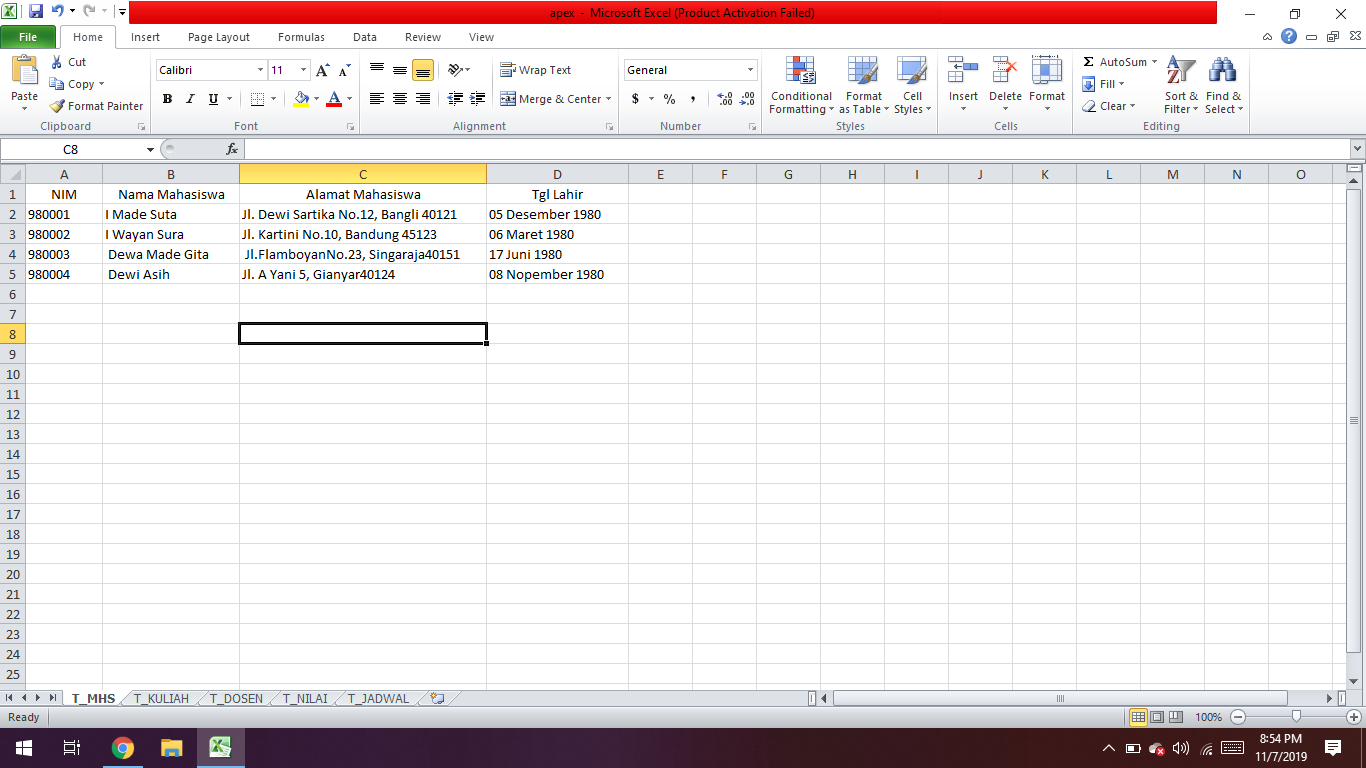
\includegraphics[scale=0.25]{figures/excel.png}
        \caption{Tabel Excel}
        \label{excel}
    \end{figure}
    \item Lalu buat tabel satu-satu sesuai dengan data yang sudah ada, buat dalam satu file dengan sheet yang berbeda.
\end{enumerate}

\section{Normalisasi Data di Apex}
\begin{enumerate}
    \item Masukkan data yang sudah ada ke dalam apex anda sesuai dengan sheetnya seperti pada gambar \ref{apex1} berikut klik app builder lalu klik Create.
        \begin{figure}[!htbp]
        \centering
        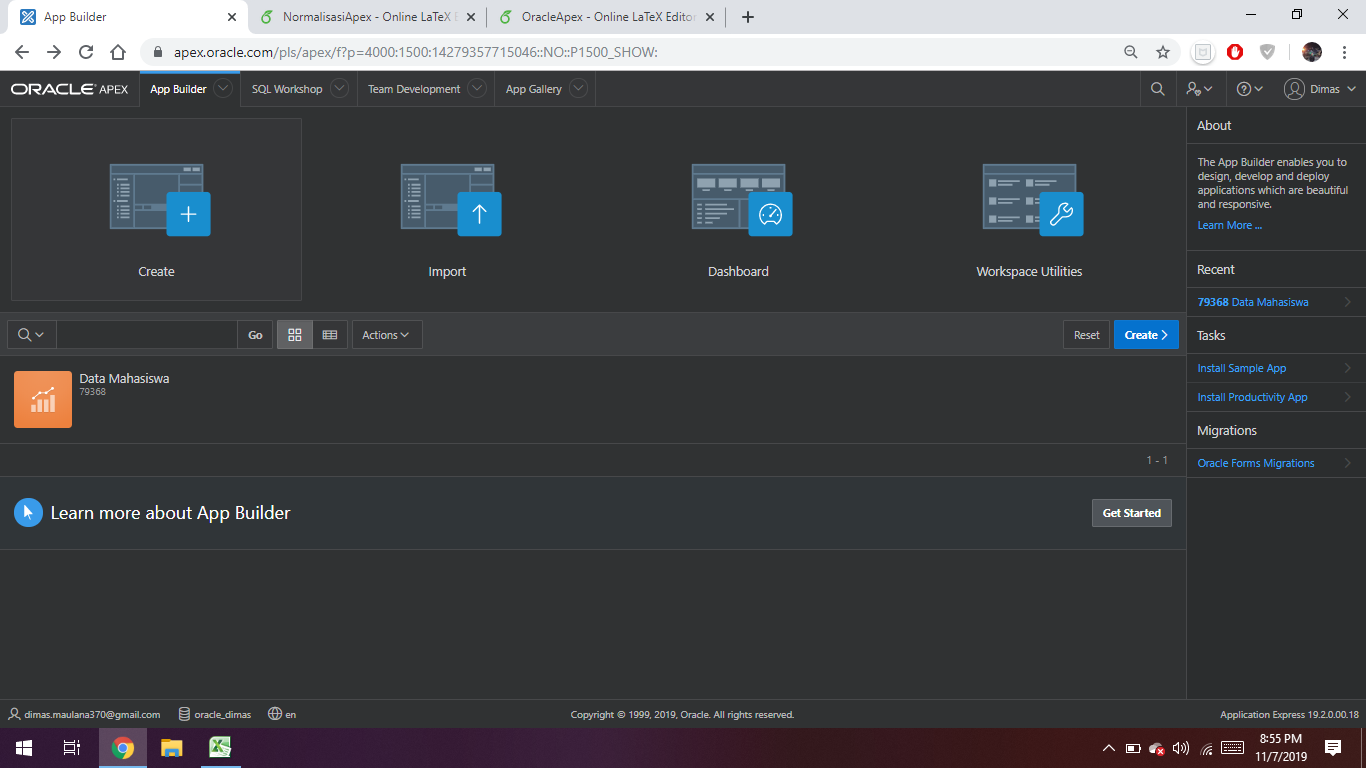
\includegraphics[scale=0.31]{figures/apex1.png}
        \caption{Memasukkan Data ke Apex}
        \label{apex1}
    \end{figure}
    \item Setelah itu klik From a File dan pilih data excel yang sudah dibuat pertama kali seperti pada gambar \ref{apex2} berikut.
            \begin{figure}[!htbp]
        \centering
        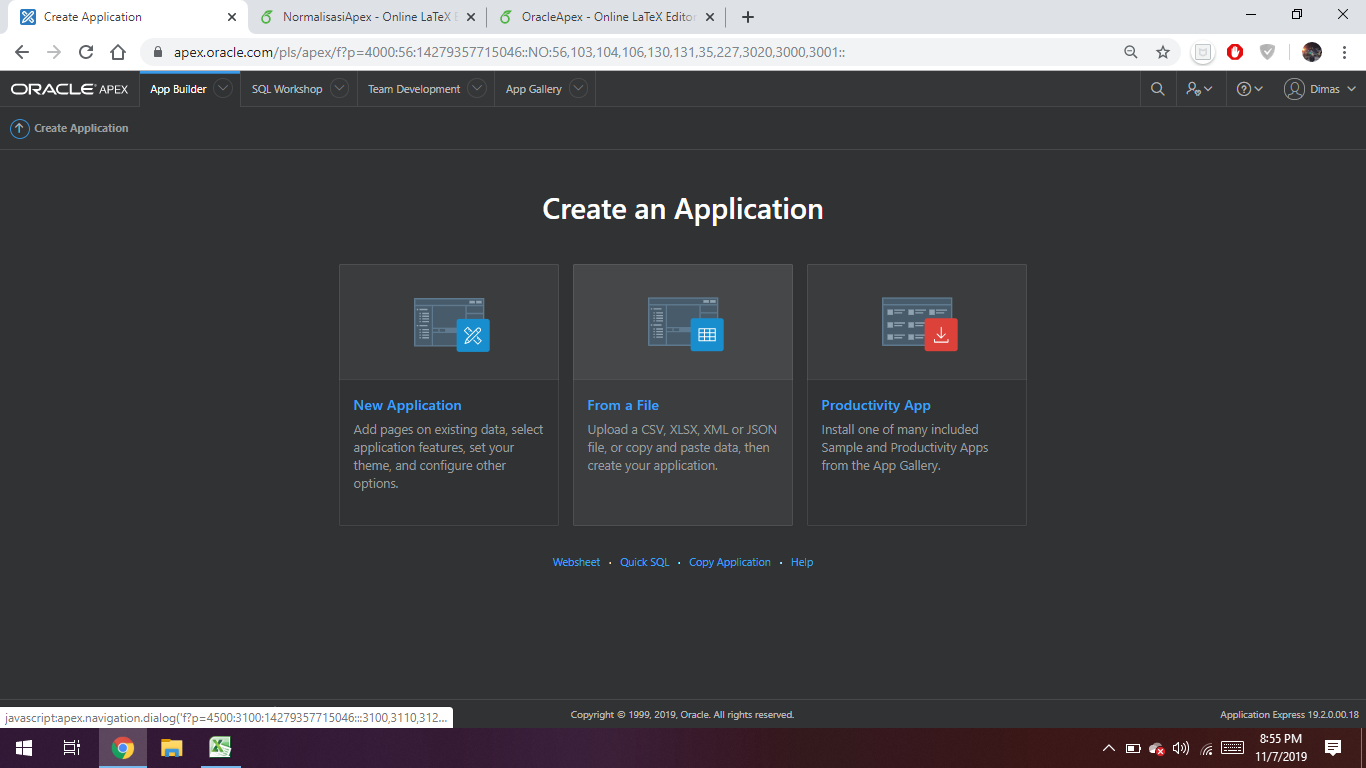
\includegraphics[scale=0.25]{figures/apex2.png}
        \caption{Memasukkan Data ke Apex}
        \label{apex2}
    \end{figure}
    \item Lalu drag atau drop file excel tadi pastikan data yang anda inputkan sesuai dengan yang anda buat pertama kali seperti pada gambar \ref{apex3} berikut.
            \begin{figure}[!htbp]
        \centering
        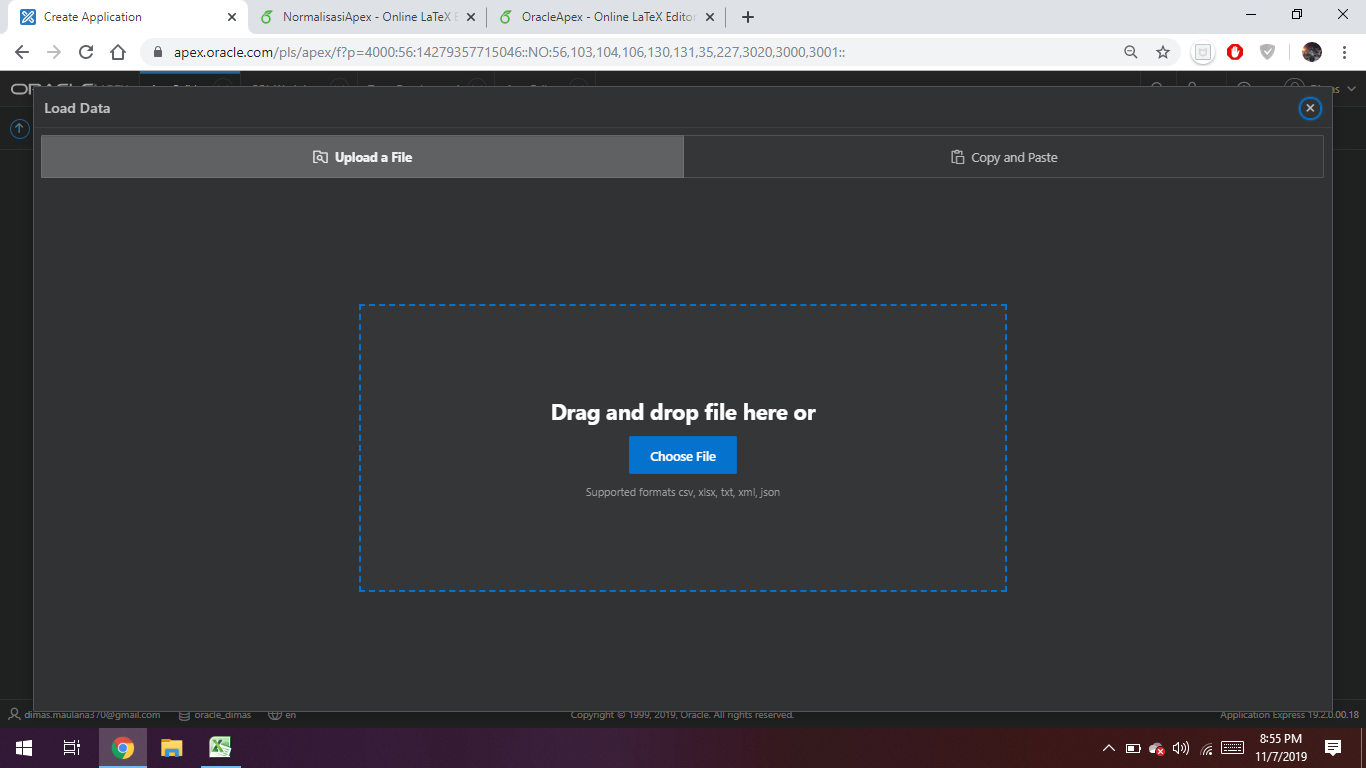
\includegraphics[scale=0.25]{figures/apex3.png}
        \caption{Memasukkan Data ke Apex}
        \label{apex3}
            \end{figure}
    \item Beri nama pada tabel yang akan di Load datanya, jangan lupa untuk memilih sheet sesuai dengan data yang bersangkutan seperti pada gambar \ref{apex4} berikut.
            \begin{figure}[!htbp]
        \centering
        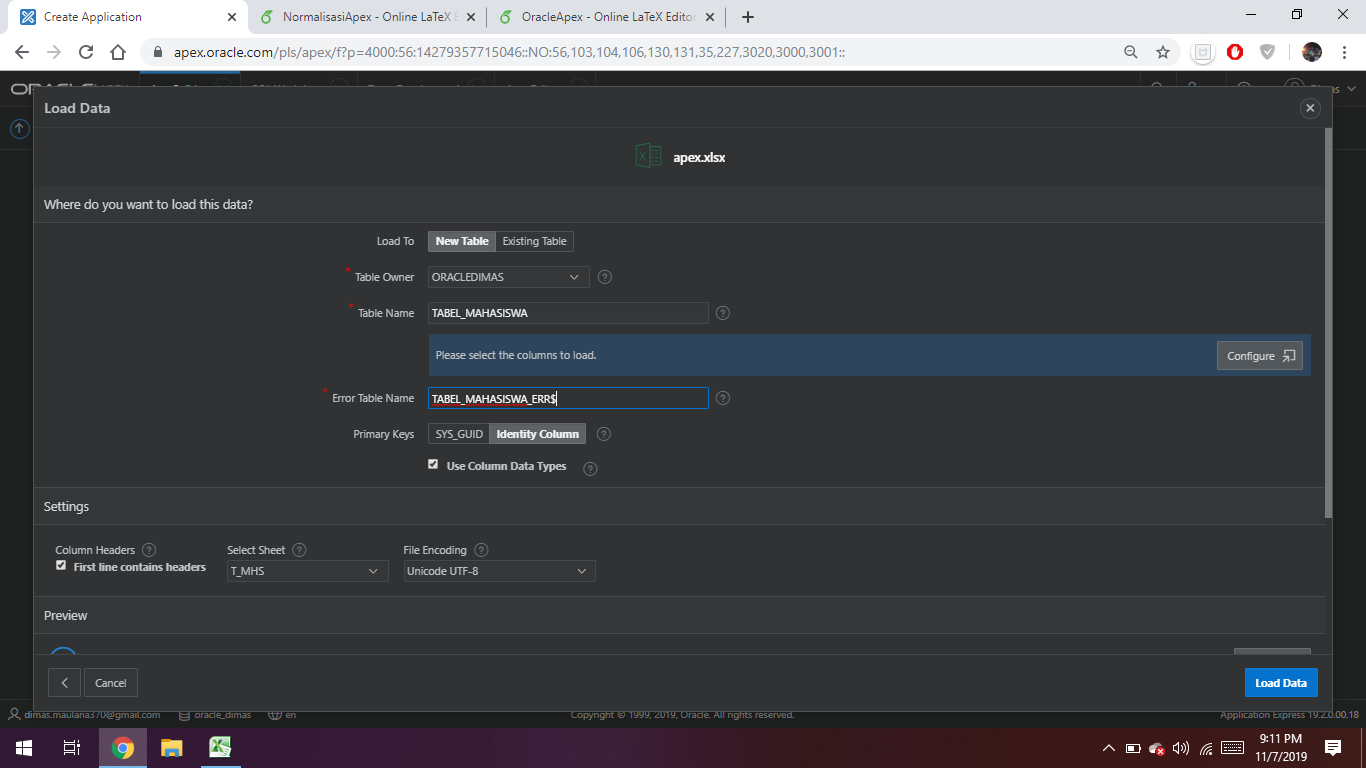
\includegraphics[scale=0.28]{figures/apex4.png}
        \caption{Memasukkan Data ke Apex}
        \label{apex4}
    \end{figure}
    \item Setelah menklik load data ulangi langkah diatas sampai semua sheet sudah dipakai lalu jangan langsung create aplikasi tetapi lanjut kelangkah berikutnya.
    
    \item Lalu masuk kedalam SQL Workshop untuk meng edit tabel-tabel yang sudah dimasukkan tadi seperti pada gambar \ref{apex5} berikut.
                \begin{figure}[!htbp]
        \centering
        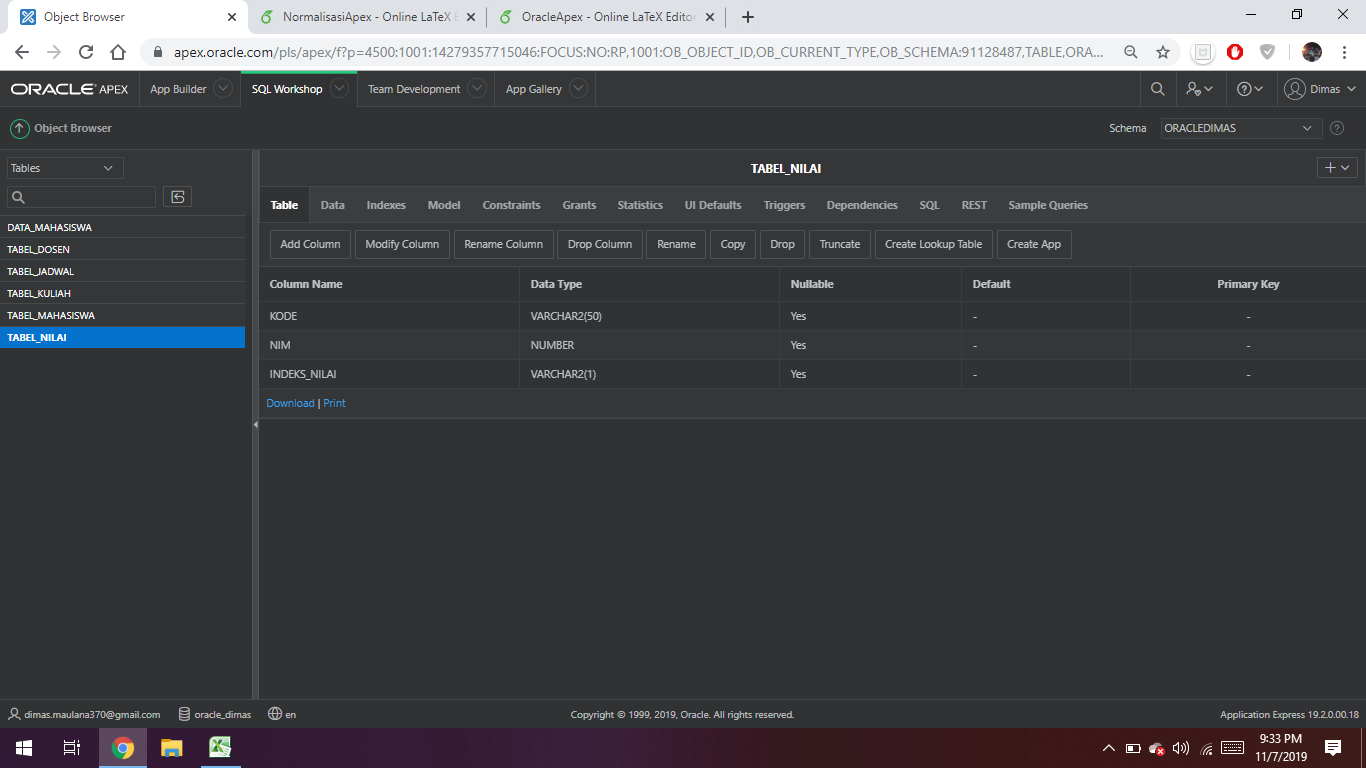
\includegraphics[scale=0.25]{figures/apex5.png}
        \caption{Mengedit Data ke Apex}
        \label{apex5}
    \end{figure}
    
    \item Apex dengan otomatis membuatkan ID untuk menjadikan primary key, maka kita harus menghapus ID tersebut karena tidak berelasi dengan tabel yang kita buat dengan cara drop column lalu pilih yang mau kita hapus.

    \item Setelah selesai menghapus semua IDnya kita jadikan setiap tabel primary key sesuai dengan yang dibutuhkan dengan cara ke SQL Comands dan isikan Query seperti pada gambar \ref{apex6}
    berikut isikan query yang sama pada tabel yang lain untuk menjadikan primary key.
    \begin{figure}[!htbp]
        \centering
        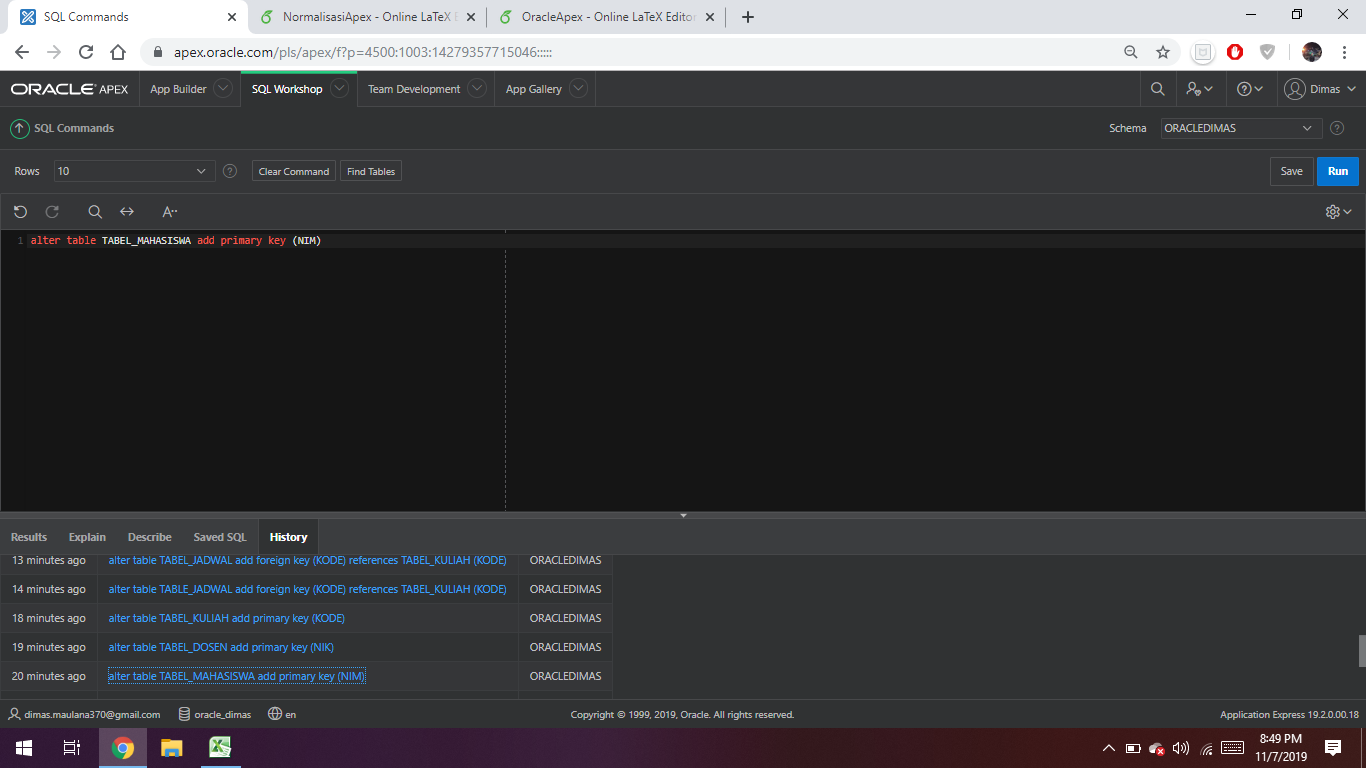
\includegraphics[scale=0.25]{figures/apex6.png}
        \caption{Normalisasi Data}
        \label{apex6}
    \end{figure}
    \item Lalu isikan Query untuk menjadikan Foreign Key seperti pada gambar \ref{apex7} berikut, tabel yang dijadikan foreign key adalah tabel nilai dan tabel jadwal lakukan query yang sama pada tabel yang lain.
        \begin{figure}[!htbp]
        \centering
        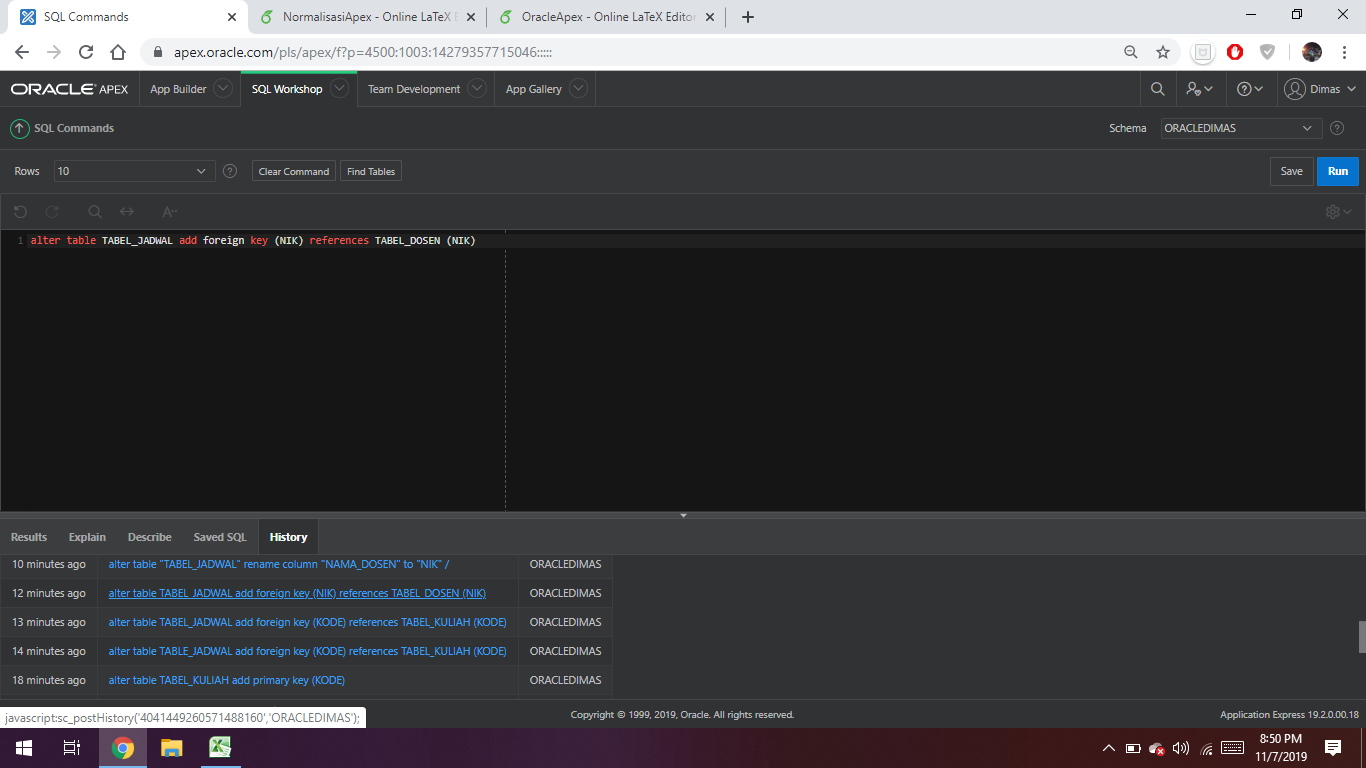
\includegraphics[scale=0.3]{figures/apex7.png}
        \caption{Normalisasi Data}
        \label{apex7}
    \end{figure}
\end{enumerate}

\section{Pembuatan Aplikasi}
\begin{enumerate}
    \item Setelah selesai menormalisasi data langkah berikutnya adalah membuat aplikasi yaitu dengan cara app builder - create - new application seperti pada gambar \ref{apex8} berikut.
            \begin{figure}[!htbp]
        \centering
        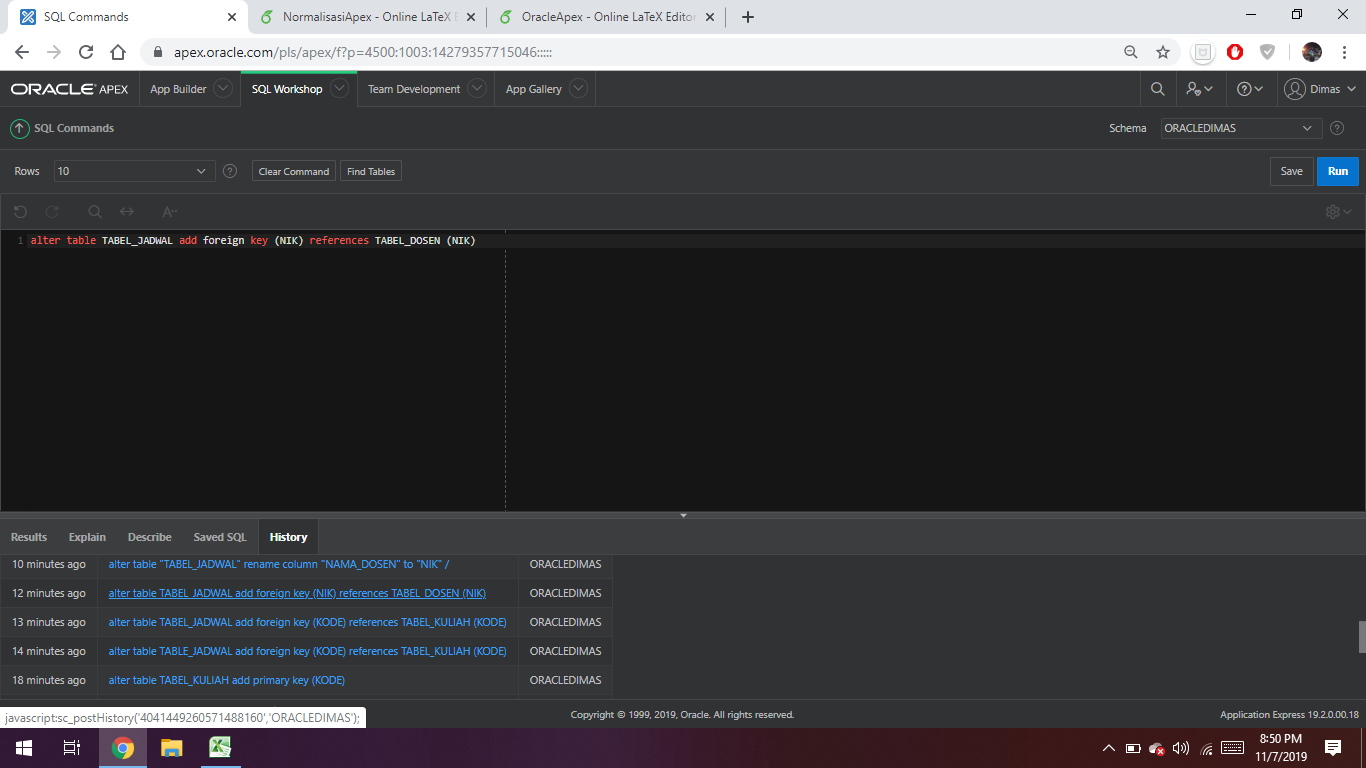
\includegraphics[scale=0.25]{figures/apex7.png}
        \caption{Pembuatan Aplikasi}
        \label{apex8}
    \end{figure}
    \item Lalu klik Add page dan pilih Interactive Report seperti pada gambar \ref{apex9} berikut.
                \begin{figure}[!htbp]
        \centering
        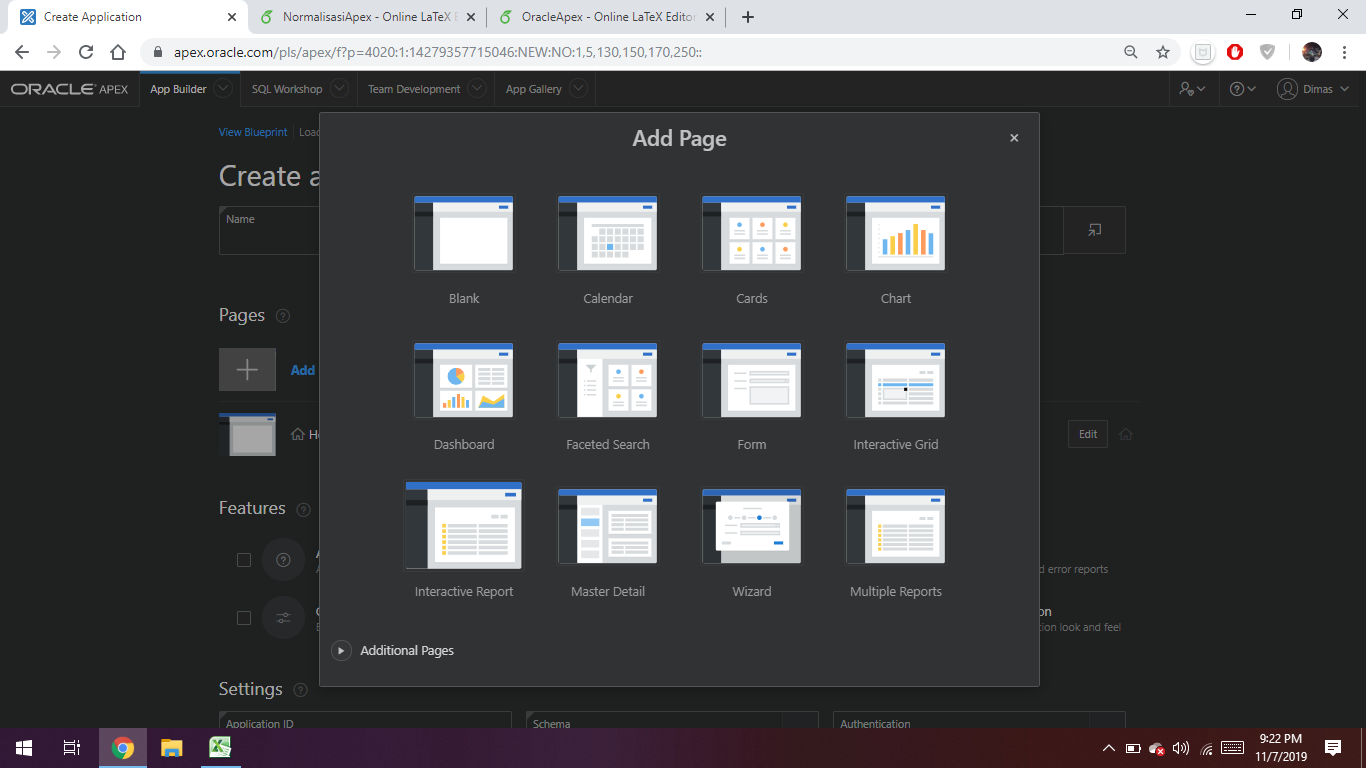
\includegraphics[scale=0.25]{figures/apex9.png}
        \caption{Pembuatan Aplikasi}
        \label{apex9}
    \end{figure}
    \item Setelah itu isikan Page Name dan pilih tabel yang berhubungan di Table of View Seperti pada gambar \ref{apex10} berikut lalu klik add page.
                    \begin{figure}[!htbp]
        \centering
        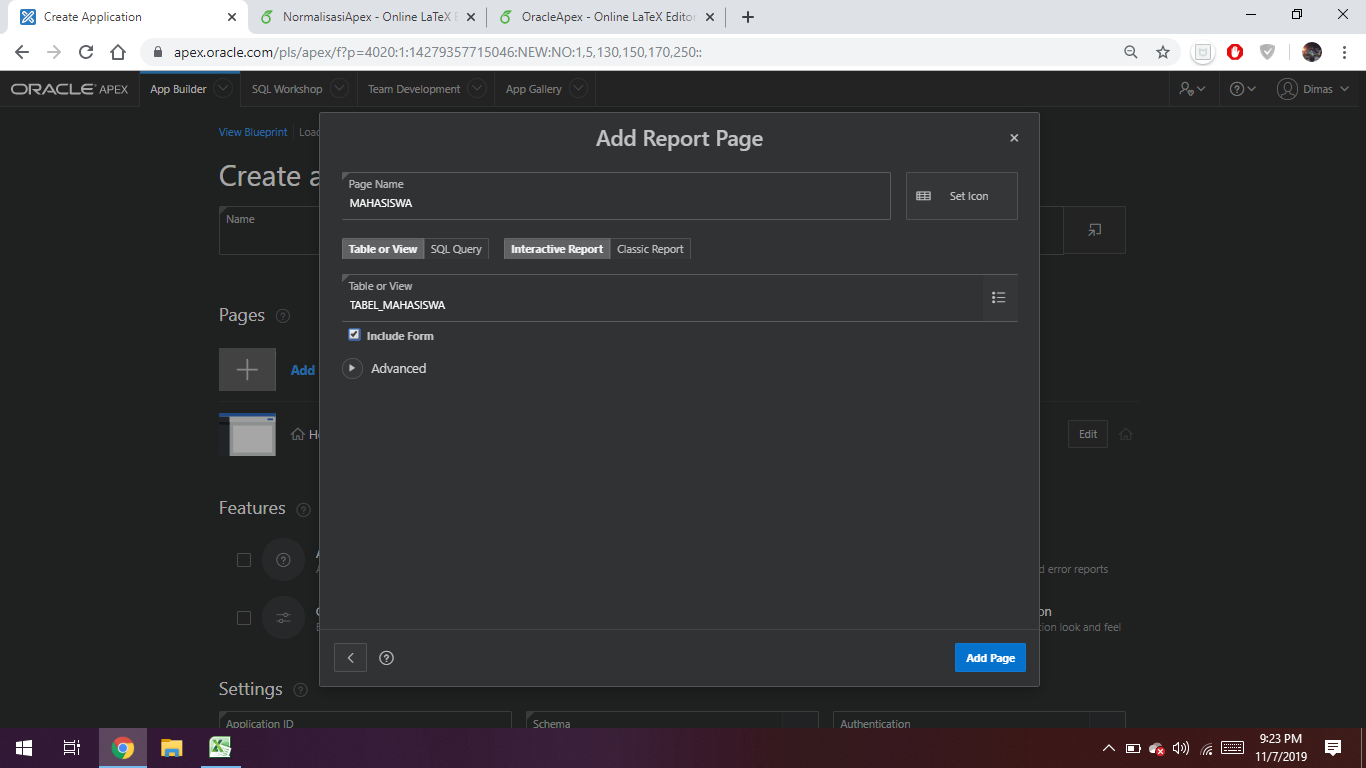
\includegraphics[scale=0.25]{figures/apex10.png}
        \caption{Pembuatan Aplikasi}
        \label{apex10}
        \end{figure}
    \item Lakukan langkah diatas berulang kali sampai ke lima data tersebut terbuat page nya.
    
    \item Langkah terakhir yaitu klik Create Application seperti pada gambar \ref{apex11} maka aplikasi kalian sudah selesai dibuat.
                    \begin{figure}[!htbp]
        \centering
        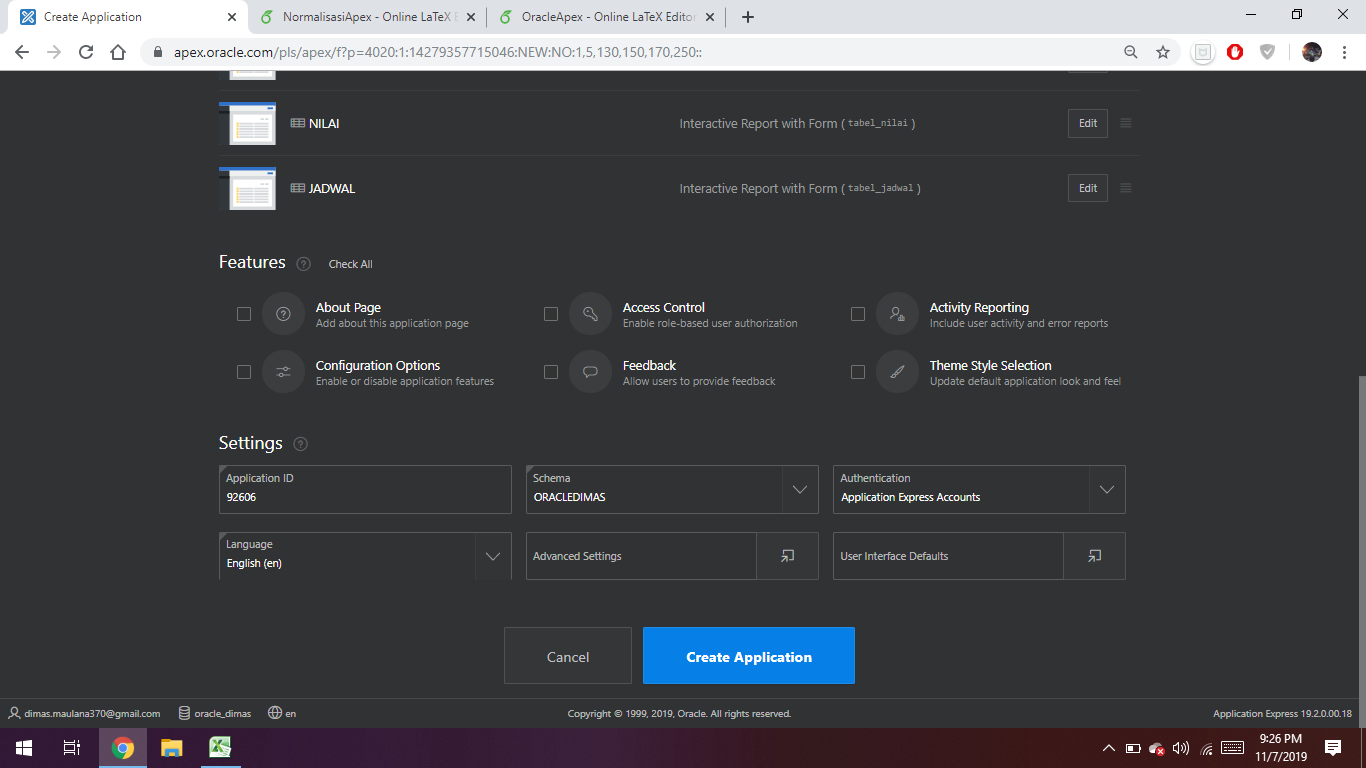
\includegraphics[scale=0.25]{figures/apex11.png}
        \caption{Pembuatan Aplikasi}
        \label{apex11}
    \end{figure}
\end{enumerate}

\section{Workspace, Email, Password, dan Site Oracle Apex}
Workspace   : ORACLE-DIMAS
\\
Email       : dimas.maulana370@gmaail.com
\\
Password    : redial24
\\
Site        : https://apex.oracle.com/pls/apex/f?p=92606:LOGIN\_DESKTOP:15524758594935:::::
\end{document}
